%Tikz-Graph Examples 
%Author: n
\documentclass{article}
\usepackage[utf8]{inputenc}
\usepackage[upright]{fourier} 
\usepackage{multicol, graphicx, enumerate, cancel, amsmath, amsthm, tikz, fullpage}
\usetikzlibrary{arrows,petri,topaths}
\usepackage{tkz-graph}
\title{Tikz Graphing Practice}
\author{Jonathon Sonesen}
\begin{document}
\maketitle

\section*{}
\begin{tikzpicture}[>=stealth']
\node(pseudo) at (-1,0){};
\node(0) at (0,0)[shape=circle,draw]            {$q_0$};
\node(1) at (2,0)[shape=circle,draw, double]    {$q_1$};
\node(2) at (4,0)[shape=circle,draw, double]    {$q_2$};
\node(3) at (6,0)[shape=circle,draw,double]     {$q_f$};
\path [->]
(0)        edge                      node[above] {b}   (1)
(1)        edge                      node[above] {a}   (2)
(2)        edge                      node[above] {b}   (3)
(2)        edge   [bend left=40]     node[below] {a}   (0)
(0)        edge   [loop below]       node[above] {a}   (2)
(1)        edge   [loop above]       node[above] {a}   (2)
(3)        edge   [loop above]       node[above] {a}   (2)
(pseudo)   edge   [loop above]       node[above] {a}   (2)
\end{tikzpicture}


\begin{center}
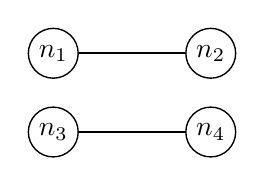
\begin{tikzpicture}[scale=1,transform shape]
%\tikzset{VertexStyle/.style={	shape = circle,							
%								fill = blue!30,
%								minimum size = 10pt,
%								draw}
%								}
\GraphInit[vstyle=Dijkstra]
\SetVertexMath

\Vertex[x=0,y=0]{n_1}
\Vertex[x=2,y=0]{n_2}
\Vertex[x=0,y=-1]{n_3}
\Vertex[x=2,y=-1]{n_4}
\Edge[](n_1)(n_2)
\Edge[](n_3)(n_4)
\end{tikzpicture}
\end{center}

\end{document}

